\documentclass[
    parskip=half, 
    twoside=false,
    twocolumn=true,
    fontsize=11pt,
]{scrarticle}
\usepackage{xcolor}
\definecolor{seeblau}{HTML}{00A9E0}
\definecolor{seegrau}{HTML}{9AA0A7}

\definecolor{seeblau1}{HTML}{CCEEF9}
\definecolor{seeblau2}{HTML}{A6E1F4}
\definecolor{seeblau3}{HTML}{59C7EB}
\definecolor{seeblau4}{HTML}{00A9E0}
\definecolor{seeblau5}{HTML}{008ECE}


\usepackage{graphicx}
\usepackage{amsmath}
\usepackage{subcaption}
\usepackage{wrapfig}
\usepackage[english]{babel}
\usepackage{blindtext}
\usepackage{microtype}
\usepackage{siunitx}
\usepackage[utf8]{inputenc}
\usepackage{csquotes}
\usepackage{nicefrac}
\usepackage[T1]{fontenc}
\usepackage{amsfonts}
\usepackage{amssymb}
\usepackage{tikz}

\usepackage{siunitx}

\usepackage{libertinus, libertinust1math}
\usepackage{roboto}

\setkomafont{disposition}{\normalfont\sffamily}


% not recommended with KOMA-script
% make table of contents sans-serif
% \usepackage{tocloft}
% \renewcommand\cftchappagefont{\normalfont}
% \renewcommand\cftchapfont{\normalfont}
% \renewcommand\cftchappresnum{\bfseries}
% \renewcommand\cftchapaftersnum{}
% \renewcommand{\cftchapfont}{\sffamily}
% \renewcommand{\cftsecfont}{\sffamily}
% \renewcommand{\cftsubsecfont}{\sffamily}
% \renewcommand{\cftchappagefont}{\sffamily}
% \renewcommand{\cftsecpagefont}{\sffamily}
% \renewcommand{\cftsubsecpagefont}{\sffamily}

% caption
\usepackage{caption}
\captionsetup{
	% font={sf},
	labelfont={sf, bf, color=seeblau},
	labelsep=quad,
	labelformat=simple,
}

% links
\usepackage{hyperref}
\hypersetup{
	colorlinks=true,
	linkcolor=seeblau,
	citecolor=seeblau,
	urlcolor=seeblau,
	% hidelinks=true
}

% bibliography
\usepackage[
	style=numeric-comp, % comp = compressed 4,5,6,7 -> 4-7
	sorting=none,		% Sort by appearance
	% autocite = superscript,
	% backref=true,
	hyperref=true,
	url=true,
	maxbibnames=100
]{biblatex}
\DefineBibliographyStrings{english}{%
    backrefpage  = {see p.}, % for single page number
    backrefpages = {see pp.} % for multiple page numbers
}

% remove issue
\AtEveryBibitem{%
  \clearfield{number}
}

\usepackage{float}
% \floatplacement{figure}{h}
% \floatplacement{table}{H}

% loosen float placement rules
\renewcommand{\topfraction}{0.8}
\renewcommand{\bottomfraction}{.8}
\renewcommand{\textfraction}{0.1}
\renewcommand{\floatpagefraction}{.9}
% make floats less likely to be placed on a separate page
\setcounter{totalnumber}{9}
\setcounter{topnumber}{9}
\setcounter{bottomnumber}{9}

% decrease space between floats and text
\setlength{\textfloatsep}{0.5cm}
\setlength{\floatsep}{0.5cm}


\usepackage{adjustbox}

\usepackage{datetime}
\newdateformat{dotdate}{
	\twodigit{\THEDAY}.\twodigit{\THEMONTH}.\THEYEAR
}
\newdateformat{monthyeardate}{%
  \monthname[\THEMONTH] \THEYEAR}


% header and footer
\usepackage[
  markcase=noupper
]{scrlayer-scrpage}% activates pagestyle scrheadings automatically
\clearpairofpagestyles
\setkomafont{pageheadfoot}{\normalfont\sffamily}
\setkomafont{pagenumber}{\normalfont\sffamily}
% \chead*{\color{seegrau} Draft \dotdate\today}
\ofoot*{\pagemark}
\ohead*{\rightmark}


\usepackage{ifthen}
\newcommand{\markieren}[4]{
    \ifthenelse{\equal{#1}{}}{}{\adjustbox{padding=3pt, bgcolor=seeblau1, margin=-1pt}{\strut{\sffamily\robotoMedium{#1}}}\\}
    \ifthenelse{\equal{#2}{}}{}{\adjustbox{padding=3pt, bgcolor=seeblau2, margin=-1pt}{\strut{\sffamily\robotoMedium{#2}}}\\}
	\ifthenelse{\equal{#3}{}}{}{\adjustbox{padding=3pt, bgcolor=seeblau3, margin=-1pt}{\strut{\sffamily\robotoMedium{#3}}}\\}
	\ifthenelse{\equal{#4}{}}{}{\adjustbox{padding=3pt, bgcolor=seeblau4, margin=-1pt}{\strut{\sffamily\robotoMedium{#4}}}}
}

\addbibresource{literature.bib}

\begin{document}

\title{title}
\subtitle{subtitle}
\author{Aurel Müller-Schoenau, Leon Oleschko}
\date{\dotdate\today}


% make a custom title page
\begin{titlepage}
    \sffamily
    \vspace*{3cm}
    {
        \fontsize{32}{32}
        \markieren{}{}{Earth Field}{Nuclear Magnetic Resonance}
    }
    \vspace{.25cm}\\
    {
        \Large
        Aurel Müller-Schoenau, Leon Oleschko\\
        Supervised by Stefan Kraner
        \vspace{.05cm}\\
        18.12.2024
        \vspace{.25cm}\\
        \normalsize
        Physikalisches Fortgeschrittenenpraktikum 2\\
        Universität Konstanz
    }
    \vfill
    {
        \normalfont\normalsize
        We demonstrated key measurements using Nuclear Magnetic Resonance (NMR) with the Earth's magnetic field. Phenomena such as Free Induction Decay and Spin Echo were explored, and relaxation constants $T_1$ and $T_2$ were determined for various samples. Imaging techniques effectively differentiated saltwater from tap water using relaxation contrast, highlighting the method's potential for non-invasive material characterization.
    }
    \vfill
    \begin{flushright}
        Available at \url{www.github.com/leoole100/fp2}.
    \end{flushright}
\end{titlepage}

\section{Introduction}
Nuclear Magnetic Resonance measurements have various applications, ranging from precise magnetic field measurements to sample identification and even imaging in medical appliances. This experiment provides an introduction of the basic concepts behind NMR and how to apply them practically. In the final section we will use the acquired knowledge to capture a cross section image of a sample containing two different substances and determine which is which.

\section{Methods}
The key principle behind the Nuclear Magnetic Resonance measurement is that a nucleus that possesses a magnetic moment which if not aligned with an external magnetic field will rotate around the magnetic field axis at its \textit{Larmor Frequency}
\begin{equation}
\label{eq:larmor_frequency}
 \omega_\text{Larmor} = \gamma B
\end{equation}
where $B$ is the magnetic flux density and $\gamma$ is the gyromagnetic ratio of the nucleus. If many nuclei oscillate coherently, the corresponding magnetic moment can be detected externally.\\
In order to detect the precession, it needs to be coherent throughout the sample.
To achieve this, the field strength $B$ must not vary significantly with position. For this experiment, the earths magnetic field is sufficient and will serve as the external field. This method is called \textit{Earth Field Nuclear Magnetic Resonance}.

\section{Results}
\subsection{Noise Analysis}
\begin{figure}
    \centering
    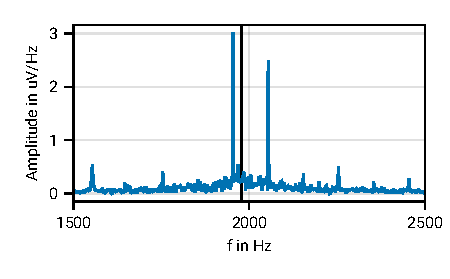
\includegraphics{figures/01 noise.pdf}
    \caption{Signal level detected by the coil for varying resonance frequency $\omega_{\text{LCR}}$ of the LCR circuit by altering the value of $C$. The yellow curve corresponds to the relationship between these variables, $\omega_{\text{LCR}} = 1/\sqrt{LC}$. $L$ is the inductance of the detection coil.}
    \label{fig:tune_C}
\end{figure}
% \begin{figure}
%     \centering
%     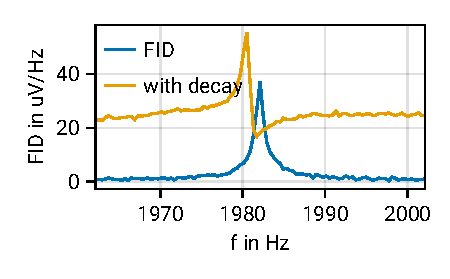
\includegraphics{figures/09 resonance.pdf}
%     \caption{
%         TODO: add to text\\
%         TODO: write caption\\
%         TODO: should we keep it?
%     }
% \end{figure}

To detect the signal later during the experiment, an electric resonant circuit of the same resonant frequency $\omega$ will be brought close to the sample. Such a circuit contains an inductance $L$ represented by a coil in the center of which the sample is located; the coil acts as the detector for the oscillating magnetic moment. A capacitor with capacitance $C$ and an ohmic resistor $R$ connected in series with the coil create an LCR circuit. Current $I$ and voltage $U$ follow a specific relationship in each of the components. For the whole circuit, this results to a second-order differential equation for $I$ and $U$ equivalent to that of a harmonic oscillator with a resonance frequency of
\begin{equation}
    \label{eq:LCR_frequency}
    \omega_{\text{LCR}} = \frac{1}{\sqrt{LC}}
\end{equation}
Given the detector coil of fixed inductance $L$, a variable capacitor can be used to tune the circuit to the larmor frequency of the sample. \autoref{fig:tune_C} shows the noise magnitude detected by the circuit with respect to variable resonant frequency following a change in $C$. The spectrum consists of a noise floor below \SI{0.1}{\micro \volt \per \hertz}, a large peak around \SI{2}{\kilo \hertz} at \SI{0.5}{\micro \volt \per \hertz} as well as a series of spikes at uneven multiples of roughly \SI{50}{\hertz}. Those spikes are likely caused by the power supply connected to the grid. The large spike might be the mechanical resonance frequency of the coil, because the magnitude increased a lot when playing a \SI{2}{\kilo \hertz} tone next to it. All other noise sources, like lamps or electronic devices and the noise generated in the measurement electronics, add up to the remaining noise floor with a RMS value of \SI{9.90}{\micro \volt \per \hertz}.

\subsection{Free Induction Decay}
\begin{figure}
    \centering
    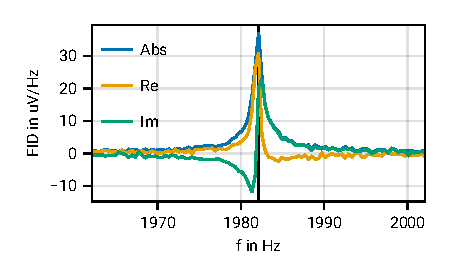
\includegraphics{figures/02 fid.pdf}
    \caption{The graph shows the complex frequency spectrum of a Free Induction Decay measurement of a water sample in the earth magnetic field. The parameters for this measurement are not optimal. Realistically, it should be possible to obtain a narrower peak that is twice as high.}
    \label{fig:FID}
\end{figure}

The goal of the first part of the experiment is to generate a macroscopic magnetic moment in the sample by applying a polarising pulse, rotating it into the plane transverse to the external field and measuring the induction voltage of the bulk moment precessing freely around the field axis. This is called \textit{Free Induction Decay}.

With no magnetic field present, the orientation of a spin does not play a role for the free energy of a system. Therefore, as long as the interaction between nuclear moments is weak, the net magnetic moment is low. In order to conduct the NMR measurement, the sample has to be polarised first by a strong external field $B_1$. This leads to Zeeman splitting of energy levels, and the sample relaxes into a state where most nuclear magnetic moments are aligned with $\vec{B_1}$ so as to minimise free energy, and the result is a macroscopic magnetisation along the polarising field. Now the polarising field is turned off. The two energy levels according to alignment or anti-alignment with the earth field, respectively, are separated by an energy difference of $\Delta E$, and a magnetic pulse at the Larmor frequency causes \textit{Rabi Oscillations} at frequency $\omega_\text{Rabi}$ between aligned and anti-aligned states. If this pulse is applied for a period of
\begin{equation}
 \tau_{\pi/2} = \frac{T_\text{Rabi}}{2} = \frac{\pi}{\omega_\text{Rabi}}
\end{equation}
the moment will be aligned orthogonally to the external field. This maximises the magnitude of the Larmor precession and therefore the Faraday induction voltage in the detection coil. The macroscopic magnetic moment is the result of many nuclear moments being aligned and precessing coherently. But this coherence is lost over time and the macroscopic moment, and therefore the signal decays gradually. This process is partially caused by dipole-dipole interaction between spins, and the according time period (this is the time after which the signal has declined by a factor of $e$) is named $T_2$. But there is another factor at play here, namely the inhomogeneity of the external field. If $B_0$ varies in space, the Larmor frequency for different nuclei will vary, causing a loss of coherence between individual nuclear moments located in places $x_1$ and $x_2$ of different flux density $B_0(x)$. The decay rate owing to field inhomogeneity
\begin{equation}
\label{eq:decoherence_inhom}
 \omega_\text{inhom.} = \Delta \omega_\text{Larmor} = \gamma (B_0(x_1) - B_0(x_2)) = \gamma \Delta B_0
\end{equation}
and the decay rate $1/T_2$ due to dipole-dipole relaxation add up to the total decay rate $1/T_2^*$:
\begin{equation}
 \frac{1}{T_2^*} = \frac{1}{T_2} + \gamma \Delta B_0
\end{equation}
A coil specifically designed to generate a gradient field can be used to compensate for the gradient of the external field and minimise the term in \autoref{eq:decoherence_inhom}. This method is called \textit{shimming}.\\
\autoref{fig:FID} shows the FID spectrum recorded for a water sample. The peak at about \SI{1980}{\hertz} corresponds to the Larmor frequency of hydrogen in the earth field, but the fact that the peak is so wide implies that the shimming parameters were not set optimally, or the resonance frequency of the detection circuit did not match $\omega_\text{Larmor}$.


\subsection{Spin Lattice Relaxation}
\begin{figure}
    \centering
    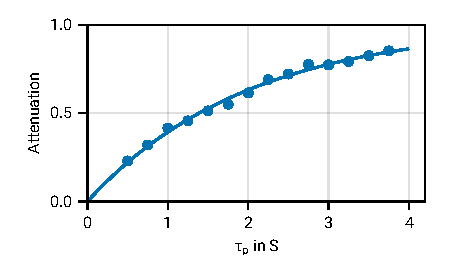
\includegraphics{figures/03 T1.pdf}
    \caption{Signal attenuation for increasing polarisation pulse duration $\tau_p$. It relaxes exponentially towards $1$ at a timescale of $T_1 = \SI{2.003(27)}{s}$. The additional oscillations owe to precession of the initial, weak bulk magnetic moment aligned with earth's magnetic field along the polarisation axis.}
    \label{fig:spin-lattice}
\end{figure}
In the previous chapter, two mechanisms were discussed which reduce the magnitude of the precessing macroscopic magnetic moment over time. Both the dipole-dipole interaction as well as the magnetic field gradient resulting in spatially varying Larmor frequencies, reduce the strength of the detected signal. But notably, \textit{both of the effects discussed above keep the bulk magnetic moment in the transverse plane} with respect to the external field. However, in order to minimise energy the moment will also change its orientation to align with the external field. This process is possible through interaction with the surrounding thermal reservoir and is called \textit{Spin-Lattice Relaxation} or Longitudinal Relaxation, because here, the component along the magnetic field axis changes. Its rate of change is proportional to the difference between it and the equilibrium magnetisation $M_0$ along the field axis:
\begin{equation}
 \frac{dM_z}{dt} = \frac{M_0 - M_z}{T_1}
\end{equation}

The time constant for Spin-Lattice Relaxation goes by the name $T_1$. Longitudinal Relaxation is the very reason the initial polarisation pulse discussed in the previous chapter even works - otherwise, the initial, weak bulk magnetic moment would simply precess around the polarisation field axis but the component along the axis would stay constant. The polarisation effect would simply not occur. \autoref{fig:spin-lattice} illustrates the effect by comparing the signal attenuation for varying polarisation pulse durations. Here, attenuation means the signal magnitude relative to the magnitude observed in case $M_z$ along the polarisation axis was equal to the equilibrium magnitude, i.e. infinite polarisation time. The graph shows the expected exponential relaxation towards an attenuation of $1$, with some additional oscillation. This is likely caused by Larmor precession along the polarisation field during the process. The longitudinal relaxation time constant $T_1$ was calculated from the fit shown in the graph. It is equal to $T_1 = \SI{2.003(27)}{s}$.

\subsection{Spin Echo}
\begin{figure}
    % \begin{subfigure}{.5\textwidth}
        \centering
        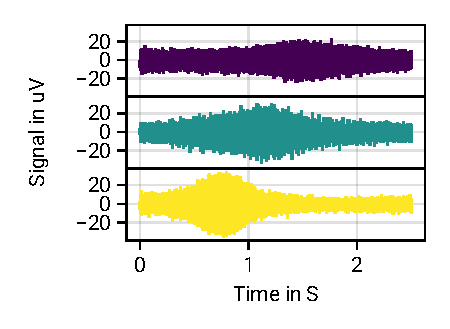
\includegraphics{figures/04 spin echo shims.pdf}
        \caption{Hahn Echo measurement for different shimming parameters. In the top graph, shimming parameters were optimised to nearly cancel out Larmor frequency variance across the sample. The resulting echo pulse is wide and shallow. In the two following examples, shimming was reduced narrowing the pulse.}
        \label{fig:hahn}        
    % \end{subfigure}
    % \begin{subfigure}{.5\textwidth}
    %     \centering
    %     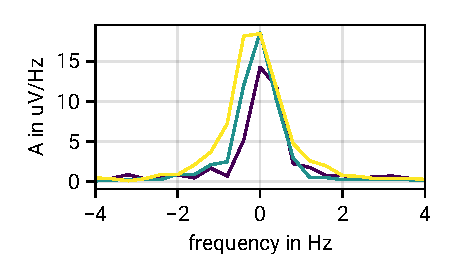
\includegraphics{figures/04 spin echo shims spectrum.pdf}
    %     \caption{TODO: should we keep it?, it doesn't look good.}
    % \end{subfigure}
    % \caption{}
 \end{figure}
A sample has been polarised by a polarisation pulse, and the magnetic moment was rotated into the transverse plane using a $\pi/2$ pulse. Now the signal induced into the detection circuit decreases due to several mechanisms. These have been discussed already, and shimming was introduced as a method of reducing decoherence caused by spatially varying Larmor frequencies. Shimming is relevant because decoherence is the strongest contributor to signal decay during Free Induction Decay. But the process is deterministic and can be reversed by applying a $\pi$ pulse to the sample. During FID a nucleus experiencing higher field strength will precess faster and obtain a positive phase difference with respect to the mean Larmor frequency precession after a time $t$. The $\pi$ pulse flips the magnetisation orientation of the nucleus in the precession plane, preserving the phase difference magnitude, but due to inverse orientation it is now negative. Once the same time period $t$ has passed again, the nucleus has overcome its phase deficiency and is now in phase with the mean precession again. The dephasing decay before the flip reverses afterwards and at time $2\cdot t$ a \textit{Hahn Echo} is observed. In \autoref{fig:hahn} the resulting echo pulse is shown for three different shimming parameters. The shortest pulse corresponds to worst shimming, resulting in fast decoherence decay and therefore a short echo pulse as phase coherence is reacquired for only a brief period of time.


\subsection{Multiple-echo experiments}
\begin{figure*}
    \centering
    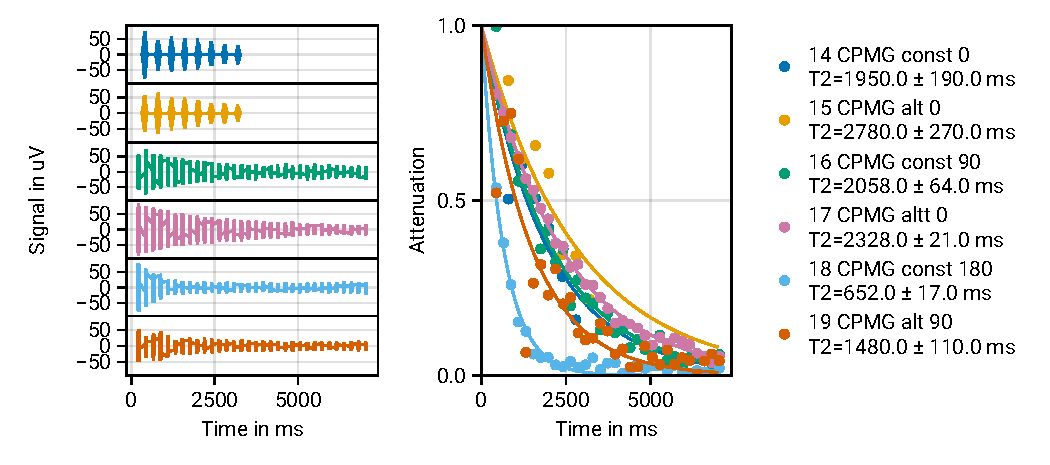
\includegraphics{figures/05 CPMG.pdf}
    \caption{CPMG pulse sequence measurement for varying phase and polarity for consecutive pulses. $T_2$ time varies because imperfect $\pi$ pulses introduce phase errors providing an additional decay channel. Slowest decay is achieved by either varying the phase by \SI{90}{\degree} each time, meaning consecutive $x$ and $y$ rotations, or by inversing pulse polarity between pulses to make phase errors cancel out. The worst result is observed for constant polarity and phase variation of \SI{180}{\degree} -- each flip occurs around the same axis and all phase errors add up!}
    \label{fig:CPMG}
\end{figure*}
If phase decoherence in the sample occurs very quickly relative to the timescale of all remaining relaxation mechanisms, echo pulses get narrow and the process explained in the previous section can be repeated many times before the signal dies down. \autoref{fig:CPMG} shows the data obtained from a series of multiple-echo measurements. Many echo pulses occur during a short period of time and the amplitude envelope shows exponential decay once again. But the time constant changes for different measurements, implying the presence of an additional decay component that depends on the echo sequence parameters. Indeed, the starting phase of consecutive $\pi$ pulses is varied and the pulses may be applied with alternating polarity when conducting a \textit{CPMG Pulse Sequence Measurement}. Imperfect $\pi$ pulses result in additional phase errors which accumulate over time. Varying phase and polarity of the pulses can omit these errors. Altering the phase by \SI{90}{\degree} between pulses ('CPMG const 90') corresponding to consecutive flips around two orthogonal axis in the transverse plane yielded a $T_2$ time of more than two seconds - nearly as good as simply altering polarity, which results in errors cancelling out every other pulse. The two methods yielded $T_2$ times of \SI{2058 \pm 64}{\milli \second} and \SI{2328 \pm 21}{\milli \second}, respectively.

\subsection{Relaxation Time Contrast}
\begin{figure}
    \centering
    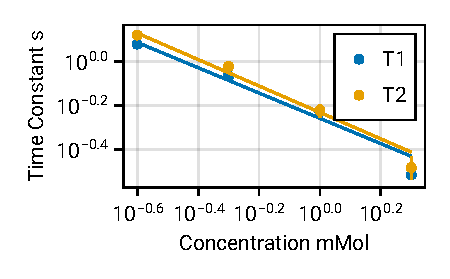
\includegraphics{figures/06 contrast.pdf}
    \caption{$T_1$ and $T_2$ times obtained from a measurement series of water samples with varying $\text{CuSO}_4$ concentration. Both axis are plotted logarithmically. The time constants get smaller as concentration increases.}
    \label{fig:CuSO4}
\end{figure}
For the final part of the experiment we will take a look at NMR imaging. This means the signal is obtained separately for different positions in space. The procedure that enable this will be explained in the following chapters.\\
But in order to acquire an NMR image in the first place, signal intensity needs to change as a function of space. This is naturally the case if spin density varies throughout the sample. If variation is relatively small within the region of interest, a contrast agent may be added to increase ('positive contrast') or decrease ('negative contrast') signal amplitude in the region of interest by altering the samples $T_1$ and $T_2$ times. An increase in $T_2$ results in a signal which persists for longer, whereas an increase in $T_1$ reduces the samples response during the polarisation, reducing the signal. Whether this results in positive or negative contrast depends on the polarisation and echo times. \autoref{fig:CuSO4} shows results obtained from a measurement series of several samples of Copper Sulfate solution with varying concentration. Both the $T_1$ and $T_2$ time constants decrease with higher $\text{CuSO}_4$ concentration.

\subsection{Imaging}
\begin{figure*}
    \centering
    \begin{subfigure}[c]{.45\textwidth}
        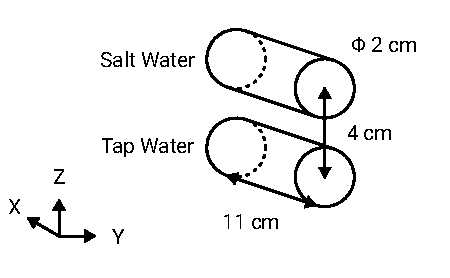
\includegraphics{figures/07 sample holder.pdf}
        \caption{A sample consisting of two tubes containing tap water and a salt water solution, respectively underwent our NMR imaging experiment. The tubes are aligned along the $x$ and $y$ axis but are offset in $z$.}
        \label{fig:sample}
    \end{subfigure}
    \begin{subfigure}[c]{.45\textwidth}
        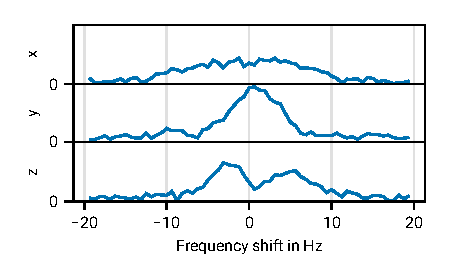
\includegraphics{figures/07 1d imaging.pdf}
        \caption{The one-dimensional image capture along the $x$, $y$ and $z$ directions resemble the structure of the two tubes: long and flat along $x$, a profile thicker towards the middle projecting onto the $y$ axis, and two distinct humps along $z$, the axis along which the samples are offset. Notice that the two humps in $z$ have different heights, because the substances in the two tubes have different NMR parameters.}
        \label{fig:1d_image}
    \end{subfigure}
    \caption{}
\end{figure*}
The spin echo measurement makes use of the fact that after inverting the phase relationship between many spins oscillating at different rates, after some time they will all align again. NMR imaging takes a more sophisticated approach: An initial gradient field $G = x G_x$ is applied to the sample. A spin at position $x$ precesses around this field over a period of time $\tau_\text{init}$ to obtain a phase of
\begin{equation*}
 \phi_X = \omega_\text{Larmor} \tau_\text{init} = \gamma x G_x \tau_\text{init} =: k_p x
\end{equation*}
The transverse magnetisation in the sample is now given by
\begin{equation*}
 M_\bot(x) = |M_\bot(x)|\cdot \exp(i k_p x)
\end{equation*}
Because the spacial position $x$ is encoded in the phase information, this is referred to as \textit{phase encoding}. The signal aquired by the detection coil is now given as the integral over all positions $x$:
\begin{equation}
\label{eq:1d_imag}
 S(k_p) = \int |M_\bot(x)| \cdot \exp(i k_p x) dx
\end{equation}
Therefore, the signal magnitude with respect to $k_p$ which depends on the field gradient, resembles the Fourier transform of the spacial magnetisation distribution in the sample along the $x$ axis. Obtaining data for many $k_p$ now allows reconstruction of $|M_\bot(x)|$ by applying IFT.\\

A sample similar to \autoref{fig:sample} was measured using this method along three spacial axis: $x$ being the axis along the cylinders, and $z$ being the axis along which the two tubes are displaced. One tube contained water while the other one was a salty solution. The image data shown in \autoref{fig:1d_image} resembles the one-dimensional structure of the sample: The distribution is roughly constant along $x$, both tubes align along the $y$ axis resulting in just one peak, and the $z$ measurement shows two seperate humps of different magnitude, owing to the different substances in the two tubes.

It is also possible to capture two-dimensional images using NMR. To do this, an additional gradient field is applied in $y$ direction \textit{during readout}. This way, a range of $k_y$ wave vectors is sampled over time. The phase for a spin at position $y$ now oscillates during readout according to $\phi_y = \gamma G_y y t := \omega_y t$. Magnetisation in $y$ is therefore encoded in the signal time domain at frequency $\omega_y$. This is called \textit{frequency encoding}. A 2d inverse Fourier Transform in $t$ and $k_p$ now yields the two-dimensional magnetisation magnitude $M_\bot(x,y)$. In \autoref{fig:2d_image} you can see three images captured of the double-tube sample in the $x$-$y$-plane. Each image was captured using different parameters. For short polarisation time, only the salt water sample shows up in the image (positive contrast) because it gets polarised quickly due to short $T_1$ time. In the second image, long polarisation time allows the water sample to also get polarised and both show up. For long polarisation time, the short $T_2$ time of the salt water sample has led to such drastic signal decay during the long acquisition delay that only the water sample shows up (negative contrast).

\begin{figure*}
    \centering
    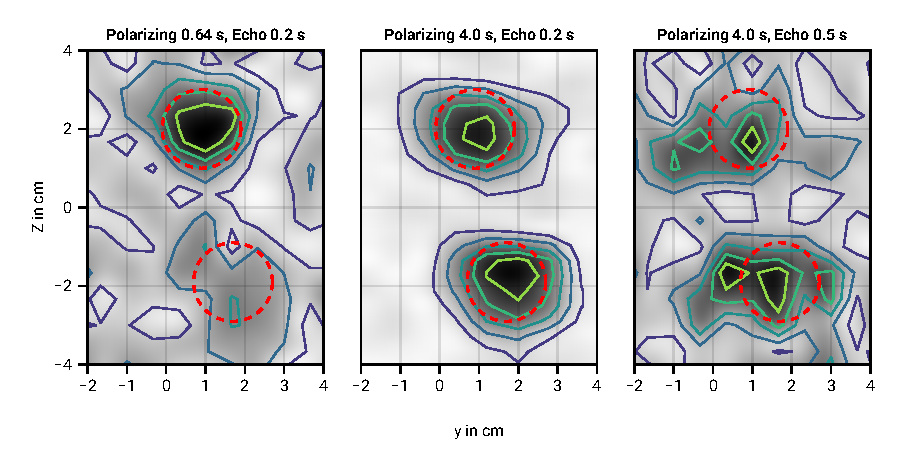
\includegraphics{figures/08 2d imaging.pdf}
    \caption{Two-dimensional image captured of the sample shown in \autoref{fig:sample} for differing parameters. The salt water sample's lower $T_1$ and $T_2$ times make it show up even after a short polarisation pulse as seen on the left, but after a long acquisition delay the signal has already faded as illustrated on the right.}
    \label{fig:2d_image}
\end{figure*}

\pagebreak
\section{Conclusion}
The EFNMR setup serves as a nice and illustrative experiment to investigate and understand the mechanisms behind Nuclear Magnetic Resonance probing and imaging. All parts of the experiment, from tuning the resonant circuit through measuring the decay time scales of different samples to capturing one- and even two-dimensional images were a success. The Larmor frequency spectrum measurement allowed for optimising shimming parameters to achieve uniform spin precession throughout the sample. Our measurements of the time constant for longitudinal relaxation not only show the expected exponential behaviour, but also exhibit small oscillations caused by Larmor precession around the polarising field. The Hahn Echo measurement worked as intended and so did the multi-pulse experiments, illustrating the impact that $\pi$ pulse errors have on the decay rate, and how to correct them. Through our testing of different Copper Sulfate solutions, we were able to confirm that the substance can be used as a contrast agent in NMR imaging. In the final part of the experiment, we were able to apply imaging procedures to correctly distinguish a salt water probe from a water sample using both positive and negative contrast imaging.

\addcontentsline{toc}{section}{Literature}
\nocite{*}
\printbibliography

\end{document}
